\chapter{Networks I: Protocols}

Computing devices have been in use for thousands of years, at least since the invention of the Sumerican abacus between four and five thousand years ago. Even as computers became more sophisticated, a long process culminating in the development of transistor-based digital computers, they remained specialized machines, largely for use in government or business settings. The explosion in personal computing, which has flooded the planet with billions of computers that pervade almost every aspect of society, coincided roughly with the development of computer networking and the Internet. Communicating via computers -- with friends, news outlets, vendors, banks, or even artificial intelligence systems -- has revolutionized the way the world works.

In the next two chapters, we'll learn how computer networks work, from the wires in the ground up to the more familiar technologies in a browser or email client. The Internet is one of the largest and most complex machines ever built, so we certainly won't be able to cover every aspect of it, but we'll focus on a few important topics. After reading, you should be able to tell a story about what happens when you open a website or send an email, and understand how to get under the hood and see how different pieces are working together to complete the task.

In this chapter, we'll focus specifically on the \emph{protocols} that allow computers to communicate with one another. We'll cover what a protocol is, and why detailed protocols are important for ensuring reliable networking. In the following chapter, we'll look at how these protocols work together and allow us to build large computer networks, including the global Internet.

In addition to its inherent interest, understanding networks is very practical. Many companies look for Internet Technology or IT specialists who understand how networks work. Taking a test like the Network+ certification or A+ certification allows access to these jobs. These tests are knowledge based, so you don’t need practical experience to do well on them. They qualify you for entry level positions that pay around \$50,000 a year. If you're interested in preparing for these exams, there are many books that can help you prepare. For instance, ``CompTIA A+ Certification All-in-One Exam Guide, Ninth Edition (Exams 220-901 \& 220-902).''

\section{Protocols}

Long before there were computers, there were protocols. A protocol is a set of rules and procedures that specify how two entities should interact. In particular, protocols can apply to people, in the form of social protocols. These can be simple -- for example, there is an unspoken protocol regarding shaking someone's hand -- or quite complex, as in the protocol for diplomatic exchanges between different countries. In fact, the US Department of State employs a Chief of Protocol, whose office is tasked with ensuring that visiting diplomats and heads of state are appropriately welcomed and not offended by any ``breach of protocol.''

Rather than delve into complex diplomatic protocol, let's consider the simple example: the ``handshake protocol.'' It's so easy to shake someone's hand that we might not realize how many rules and procedures we follow when we do it. Here are a few possible ``breaches of protocol'' that could occur when Alice shakes Bob's hand.
\begin{itemize}
    \item Alice extends a left hand, while Bob extends a right hand.
    \item After locking hands, Alice refuses to let go for a full 15 seconds.
    \item After locking hands, Alice lets go immediately without pausing for a shake.
    \item Alice refuses to make eye contact for the duration of the handshake.
    \item Alice shakes her hand left to right, or forward and backward.
    \item Alice makes no effort to grip Bob's hand, leaving the handshake loose.
    \item Alice uses a ``death grip,'' causing Bob discomfort.
    \item Alice extends her arm fully and locks her elbow, keeping Bob at as great a distance as possible.
    \item Alice barely extends her arm, forcing Bob to stand very close.
    \item Alice sneezes into her hand immediately before initiating the handshake.
\end{itemize}
Any of these examples would cause some problems; many would lead Bob to wonder if Alice had ever shaken hands before, while a few might leave Bob offended or wondering if Alice is interested in communicating. Clearly it is important that Alice and Bob abide by some rules so that their handshake goes smoothly and gives a friendly message to both parties.

How might we construct such a set of rules, or a protocol? It would be helpful to first divide the above gaffes into a few categories. We could do this chronologically: there are potential problems with initiating the handshake, completing the handshake itself, and terminating the handshake.

Let's first write a protocol for initiating a handshake. The two parties need to come to an appropriate distance, verify that their hands are clean, make eye contact, and both extend the same hand. We can condense this into a step-by-step procedure:

\begin{graybox}
{\Large Handshake Initiation}
\begin{enumerate}
    \item Verify that your right hand is acceptably clean, and maintain this status until handshake termination.
    \item Look at the other party, and wait for eye contact to be established.
    \item After making eye contact, approach the other party and come to within about one arm length apart.
    \item Extend your right hand to the halfway point between you and the other party, at about waist height, and orient your hand so that your open palm is facing left.
    \item Wait for the other party to extend their hand likewise.
\end{enumerate}
\end{graybox}

There are a surprising number of steps for something we all do almost unconsciously! 

\begin{exercise}
    Write similarly detailed protocols for Handshake Completion and Handshake Termination. Make sure your protocol eliminates the possibility of any of the gaffes listed above.
\end{exercise}

Computers have no social intuition whatsoever. This is why protocols are important: a computer needs to be told every single step of an interaction as simple as a handshake in order to execute it properly. Building a computer network requires a number of different protocols to establish how messages are sent on wires, routed to the appropriate destination, and more.

One of the most important parts of a protocol is that everyone follows the same one. Some aspects of protocols are completely arbitrary, and it is important for everyone to follow the same arbitrary convention. For example, handshakes could use left hands instead of right hands. Luckily the whole world shakes right hands, but anyone who's tried driving in both the US and UK knows that not all protocols are globally uniform.

In order to ensure that networking protocols are consistent around the world, a body known as the Interent Engineering Task Force (IETF) carefully specifies all the protocols and makes them publicly available. Publications of the IETF are known as Requests for Comments, or RFCs. The name ``Request for Comments'' originated in the early days of networking when the documents really were intended for discussion and subsequent revision. Nowadays there is a category called standards-track RFCs which specify the standards of the Internet and which should be followed by anyone building networking technology.

\section{Network Layers}\label{sec:network:layers}

In the previous section we saw an example of a protocol for initiating a handshake. The protocol was more detailed than you might have expected, but it also didn't include all the details. For example, let's delve into step 2: ``Look at the other party, and wait for eye contact to be established.'' First, what does it mean to ``look at the other party''? This requires identifying the location of another human, and sending motor signals to the neck and to the eyeballs in such a way as to orient them in the direction of the other human's eyeballs. If we were to include all these details, our protocol would become extremely complex and hard to follow.

In real life, we avoid this complexity by never even thinking about these details of movement, facial recognition, and the like. Our brains can automatically send the right signals to our muscles, interpret signals from our senses, and so on. We say that the brain is segmented into two layers: conscious and unconscious. The conscious layer sends high-level signals, such as the command ``Look at Bob,'' to the unconscious layer. The unconscious layer is responsible for parsing those commands and executing them by sending the right signals to muscles. This layered architecture allows the protocols to remain simple by referring to the capabilities of lower layers.

Communication networks also use a layered architecture. We will come to the layers that make up the Internet in a moment, but long before the Internet we had the postal system. The postal system is built up from layers, and in many ways the Internet is simply a much faster and more automated version of the same layers. Let's consider the following example of a letter being sent from Alice at Acme, Inc. to Bob at Boxes, Inc.:

\begin{enumerate}
    \item Alice tells her employee, Jane, to order 50 new boxes. Jane drafts a letter to Bob at Boxes, Inc.: ``Please send 50 boxes.'' She seals it in an envelope, opens her address book and copies down Bob's mailing address, and drops the envelope off at the company mailroom. A worker in the mailroom sees that the letter is addressed to a destination outside Acme, Inc., and so he places the envelope in a postal box outside.
    \item A postal worker picks up the envelop from the postal box, and sees that the letter is addressed to a location outside the city. He brings the letter to the local post office, and places it into a bin to be sorted.
    \item Another postal worker picks up the envelope from the bin, and puts it on a mail truck destined for Bob's city.
    \item The mail truck drives along a highway from Alice's city to Bob's city, and gives the letter to the post office there.
    \item A postal worker in Bob's city carries the envelope to Boxes, Inc., and places it in their mailbox.
    \item A worker in the mailroom sees the envelope addressed to Bob. She brings it to Bob's office and puts it on his desk where he'll see it.
    \item Bob reads the letter, and asks an employee to begin producing 50 new boxes for Acme, Inc.
\end{enumerate}

There's a lot going on here -- when you think about it, it's amazing that the letter managed to reach Bob at all, given everything that had to go correctly. The trick here is the layered architecture. Alice didn't need to know what highway the letter would be carried on, and the mail truck driver didn't need to know where to find Bob's address. Everyone in the pipeline has a specialty, and no one needs to understand the full process for it to work well. Figure \ref{fig:layer_mail} shows the different steps arranged in layers, from Alice and Bob at the top down to the truck driver at the bottom.

\begin{figure}
    \centering
    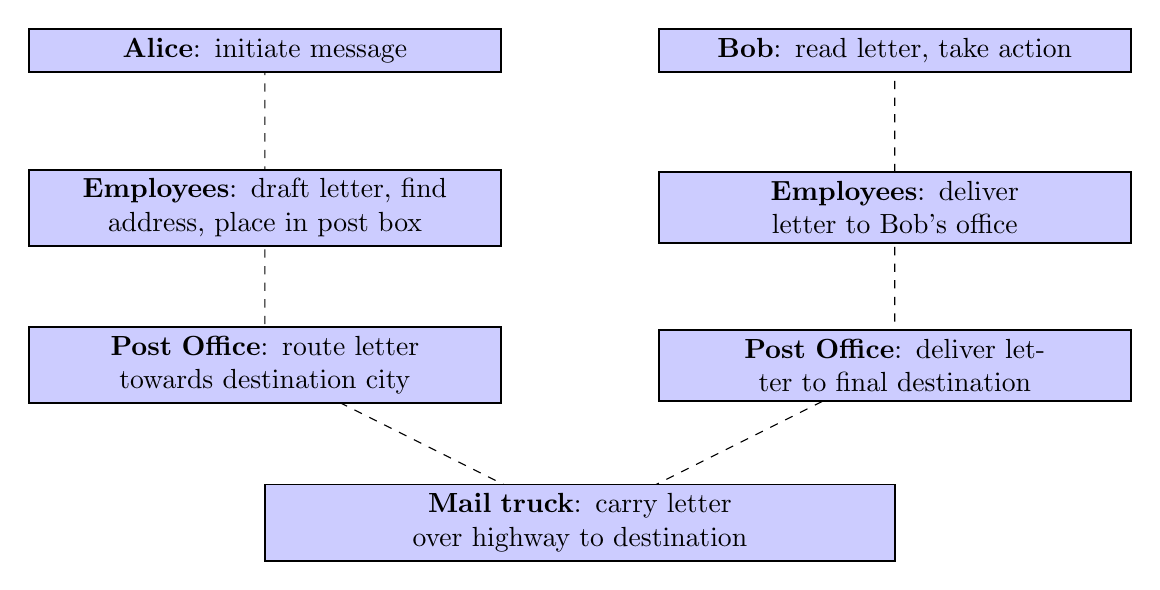
\begin{tikzpicture}[layer/.style={fill=blue!20,minimum width=6cm,align=center,text width=5.5cm,draw=black,solid,line width=.25mm}]
        \draw[dashed,-latex] (-4, 4) node[layer] {\textbf{Alice}: initiate message} --
        (-4, 2) node[layer] {\textbf{Employees}: draft letter, find address, place in post box} --
        (-4, 0) node[layer] {\textbf{Post Office}: route letter towards destination city} --
        (0, -2) node[layer,minimum width=8cm,text width=7.5cm] {\textbf{Mail truck}: carry letter over highway to destination} --
        (4, 0)  node[layer] {\textbf{Post Office}: deliver letter to final destination} --
        (4, 2)  node[layer] {\textbf{Employees}: deliver letter to Bob's office} --
        (4, 4)  node[layer] {\textbf{Bob}: read letter, take action};
    \end{tikzpicture}
    \caption{Layers of the postal system.}
    \label{fig:layer_mail}
\end{figure}

These layers all have counterparts in the Internet. At the top, we have the \emph{application layer}: programs which rely on the Internet and know how to initiate messages, much like Alice and Bob. The application layer relies on the \emph{transport layer} to determine an address where the messages should go, just as Alice relied on Jane to find Bob's mailing address. The transport layer relies on the \emph{Internet layer} to use the address to send the message to the right location, just as the Post Office routed Alice's letter to Bob's city. Finally, the transport layer relies on the \emph{link layer} to physically transmit data over wires or wireless protocols, just as the Post Office relies on mail trucks to move envelopes.

This set of four layers is commonly known as TCP/IP, named for the Transmission Control Protocol (TCP) which commonly runs the transport layer, and the Internet Protocol (IP) which commonly runs the Internet layer. The following sections contain more details on each of the layers and the protocols they use. You should always keep in mind that these layers work together just like the layers of the postal system work together.

\subsection{Application Layer}

The application layer is the highest layer of TCP/IP. It consists of various protocols that specify how to send different types of data over the Internet. You might have heard of one of these protocols, HTTP. HTTP stands for HyperText Transfer Protocol. It comes at the beginning of a web address. When you type \ic{http://www.google.com}, you're telling your computer to use HTTP to access \ic{www.google.com}.

There are many other protocols in the application layer. HTTPS is a secure version of HTTP, which uses security protocols we'll discuss in Section \ref{sec:network:security}. Another popular protocol is SSH, or Secure Shell, which programmers use to access a Linux terminal on another Internet-connected machine. The file transfer protocol, or FTP, is used for exchanging files between different computers. A variety of protocols, such as POP3, IMAP, and SMTP, are used for exchanging emails.

When the application layer receives data from the transport layer, it needs to know which protocol it was sent with. In order to sort out all the different data, the application layer uses \emph{ports}. All Internet communications happen over some numbered port. For example, HTTP uses port 80. When you load \ic{http://www.google.com}, your computer sends the request to Google over port 80. Google sends its home page back over port 80. Table \ref{tab:common_ports} lists the most commonly used protocols and the ports they use.

\begin{table}
    \centering
    \begin{tabular}{lll}
        Protocol & Port & Usage \\
        \hline
        HTTP & 80 & Web traffic \\
        HTTPS & 443 & Secure web traffic \\
        FTP & 21 & File transfer \\
        SSH & 22 & Remote shell access \\
        IMAP & 993 & Receiving email \\
        SMTP & 587 & Sending email
    \end{tabular}
    \caption{Commonly used Internet protocols.}
    \label{tab:common_ports}
\end{table}

If you write a program that uses the Internet, you will interact primarily with the application layer. A very common example is writing a program which runs on a web server. A web server is a computer which is connected to the Internet, and runs a program that constantly listens for incoming communications on ports 80 and 443 -- the ports used for the World Wide Web. When it receives a request, it will run a program and send the output of that program back to the requester. Every website is hosted by a web server, which knows how to send the data of the website to anyone who requests it.

A simple and famous example is \ic{isitfriday.net}. This website is hosted by a server which listens for requests. When it gets a request for \ic{isitfriday.net}, it will run a program which checks if it is Friday (you'll learn how to use ``if'' logic in programs in the next chapter). If it is Friday, it sends back a website that says ``Yes.'' Otherwise, it sends back a website that says ``Not yet.''

\subsection{Transport Layer}

When the application layer is ready to transmit a message, it will pass it down to the transport layer. By far the most common transport layer protocol is TCP, for Transmission Control Protocol. We will focus on TCP in this section. Another common protocol in the transport layer is TLS, for Transport Layer Security, which runs alongside TCP. We will discuss TLS more in Section \ref{sec:network:security}.

When TCP is asked to transfer a message, it will prepare to send it piece by piece over the network. The individual pieces are called \emph{packets}. These packets are relatively small, about a kilobyte. For reference, an average-sized image would typically be broken into a few thousand packets before being transferred. 

The reason for this is that a major role of TCP is to guarantee reliability. The application layer assumes that its message will be sent in full and without errors, while the Internet layer does not guarantee accurate or successful transmission, so it is the job of the transport layer to ensure robust communication. By breaking a message into small packets, TCP helps to reduce the chance that any individual packet fails to transmit. In addition, if a packet does fail to transmit, it doesn't take too much time to recover, since TCP can re-send the relatively small packet.

In addition to providing reliability, TCP is responsible for initiating connections between two computers. When TCP receives a request to transfer a message to a destination, it will first complete a ``handshake'' with that destination. The goal of the handshake is to establish that both parties are connected to the Internet and ready and willing to communicate with one another. In addition, the parties need to synchronize a \emph{sequence number} which specifies the numbers that will label subsequent packets.

We have already thought about handshakes between humans in some detail, so now let's delve into how TCP facilitates handshakes between computers. If humans were communicating using a TCP-style handshake, the conversation might look like this:
\begin{enumerate}
    \item Alice says to Bob, ``Let's start talking. I'll send some packets, starting with this one, \#3874.''
    \item Bob says to Alice, ``I hear you Alice, and I'm looking forward to packet \#3875. My packets will start with this one, \#8452.''
    \item Alice says to Bob, ``Great, I'm looking forward to packet \#8453.''
\end{enumerate}
This is the \emph{three-way handshake} model. First, Alice notifies Bob of her intent to communicate and synchronizes her sequence number. Then Bob sends an acknowledgement of Alice's sequence number, and also synchronizes his own sequence number. Finally, Alice acknowledge's Bob's sequence number, and then they are ready to communicate.

There are two kinds of messages being sent in the handshake, synchronization and acknowledgement. These are typically abbreviated as \ic{SYN} and \ic{ACK}. The TCP handshake protocol works as follows.
\begin{graybox}
{\Large TCP Handshake}
\begin{enumerate}
    \item $A$ generates a random number $x$. $A$ sends $\boxed{\ic{SYN}\ x}$ to $B$.
    \item $B$ generates a random number $y$. $B$ sends $\boxed{\ic{ACK}\ x+1}$ to $A$, and then sends $\boxed{\ic{SYN}\ y}$ to $A$.
    \item $A$ sends $\boxed{\ic{ACK}\ y+1}$ to $B$.
\end{enumerate}
\end{graybox}

\subsection{Internet Layer}

Perhaps the most interesting layer of the TCP/IP stack is the Internet layer, which almost always consists of the Internet Protocol (IP). This layer corresponds to the Post Office in our analogy: it is responsible for routing data where it needs to go. Just as the Post Office uses mailing addresses to specify locations, the Internet layer uses IP addresses to specify computers on the network.

An IP address is a sequence of 32 bits, grouped into blocks of 8. When they are written out, the groups of 8 bits are converted to decimal numbers between 0 and 255. The groups are separated by dots, so sometimes an IP address is referred to as a ``dotted quad.'' For example, the IP address \ic{172.217.15.78} points to the server which hosts \ic{www.google.com}. These addresses are stored in a sort of phone book called the Domain Name System, or DNS. When you type a website into your browser, it will first look up its IP address in the Domain Name System, and then request that IP address over the network.

When the Internet layer receives a packet from the transport layer for transmission, it will look at the IP address of the destination. It knows how to find a server which is closer to that destination. For example, if a server in New York City sees a packet destined for an IP address in Washington, DC., it might decide to forward that packet to a server in Philadelphia, PA.

You can view this process yourself using a Unix utility called \ic{traceroute}. Open a terminal and type \ic{traceroute} followed by any website. You'll see how the Internet Protocol routes your packets through different servers in order to reach their destination. For example, below is the route from a personal computer to \ic{youtube.com}. The address in the last line, \ic{172.217.12.238}, specifies the location of one of YouTube's servers.

\label{code:traceroute}
\begin{monospace}
# traceroute youtube.com
    1  192.168.1.1 (192.168.1.1)  0.448 ms  0.958 ms  0.966 ms
    2  * * *
    3  ae1312-21.ARTNVAFC-MSE01-AA-IE1.verizon-gni.net (100.41.21.152)  7.779 ms  7.766 ms  7.628 ms
    4  0.ae10.GW13.IAD8.ALTER.NET (140.222.225.219)  9.139 ms  9.117 ms  9.082 ms
    5  72.14.218.232 (72.14.218.232)  8.507 ms  7.277 ms  4.378 ms
    6  * * *
    7  216.239.54.106 (216.239.54.106)  4.779 ms 108.170.232.0 (108.170.232.0)  12.022 ms 108.170.246.33 (108.170.246.33)  16.086 ms
    8  108.170.246.67 (108.170.246.67)  12.976 ms 108.170.232.19 (108.170.232.19)  12.769 ms 108.170.246.66 (108.170.246.66)  10.935 ms
    9  iad30s15-in-f14.1e100.net (172.217.12.238)  10.570 ms 216.239.47.127 (216.239.47.127)  16.793 ms iad30s15-in-f14.1e100.net (172.217.12.238)  10.485 ms
\end{monospace}

The IP addresses we've described all correspond to version 4 of the Internet Protocol, or IPv4. There are about four billion unique IPv4 addresses, which seemed like plenty at the time of its creation. However, the growth of the Internet and the proliferation of mobile devices has led to the exhaustion of almost all IPv4 addresses. In order to ensure that the Internet can continue to grow, a transition to IPv6, which provides for many more addresses, is slowly taking place.

In the transport layer, we delved into the step-by-step procedure used for handshaking. These sorts of procedures are one important aspect of the protocols that run networks. Another important aspect is the format in which data is sent. The link layer, which we'll come to in the next section, can only send sequences of bits -- zeroes and ones -- so it is important for both parties to agree on which bits mean what.

To give an example of this, we will look inside the packets sent by IPv4. You should not try to memorize the following, but instead try to appreciate the importance of having a detailed packet structure.

An IP packet is divided into its \emph{header} and the \emph{data}. The header contains information about how the packet is being transmitted, while the data is the actual contents of the packet. The format of IPv4 headers is shown in Table \ref{tab:ipv4}. The various segments specify the following information.
\begin{itemize}
    \item \textbf{Version}: the first four bits specify the version of IP being used. For IPv4, these bits are always \ic{0100}, binary for 4.
    \item \textbf{IHL}: this is the Internet Header Length. This specifies the number of 32 bit blocks, called ``words,'' used by the header. In Table \ref{tab:ipv4} we show a header with 5 words, so these bits are \ic{0101}. This is almost always the case, although it is possible to have a larger IHL value and include additional data in the header.
    \item \textbf{DSCP}: this stands for Differentiated Services Code Point. These bits are used to specify the type of service for the packet. This allows the network to give priority to some packets, such as those used for voice or video calling, which need to arrive as quickly as possible.
    \item \textbf{ECN}: this stands for Explicit Congestion Notification. This allows the network to flag packets which are experiencing congestion along their routes.
    \item \textbf{Total Length}: this specifies the total length of the packet, in bytes including both the header and data. Since it is 16 bits, the maximum value is $2^{16}-1 = 65535$ bytes, or about 64 KB.
    \item \textbf{Fragmentation Data}: these bits are used to group packets which have been fragmented due to a maximum transmission size imposed by the link layer.
    \item \textbf{Time to Live}: this keeps track of how many hops a packet has made through the network. Every time the packet is forwarded along a new link in the network, this value is decreased by one. If it hits zero, the packet is dropped and the sender is notified. This is how the \ic{traceroute} utility works: it sends packets with small Time to Live values, and waits for the notifications to see where the packet was after one hop, two hops, etc.
    \item \textbf{Protocol}: this specifies the transport layer protocol which is making use of IP. For example, for TCP the protocol value is set to 6.
    \item \textbf{Header Checksum}: these bits are used for correcting errors in the header. The idea of a ``checksum'' is encoded in the word: we could imagine transmitting a stream of bits, followed by a few bits that count the number of ones in the original stream. If a zero was flipped to a one, or a one was flipped to a zero, then the receiver will notice that the checksum does not match and can ask for the packet to be resent. In practice a checksum is a more complicated function of the bits, but the idea is the same.
    \item \textbf{Source IP Address}: this is the address of the device sending the packet. Note that it spans 32 bits, since an IPv4 address consists of four numbers each from 0 -- 255, which require 8 bits each.
    \item \textbf{Destination IP Address}: this is the address of the device meant to receive the packet.
\end{itemize}

\begingroup
\tabcolsep=0.05cm
\begin{table}
    \centering
    \footnotesize
    \begin{tabular}{|c|c|c|c|c|c|c|c|c|c|c|c|c|c|c|c|c|c|c|c|c|c|c|c|c|c|c|c|c|c|c|c|c|}
        \hline
        Bit & 0 & 1 & 2 & 3 & 4 & 5 & 6 & 7 & 8 & 9 & 10 & 11 & 12 & 13 & 14 & 15 & 16 & 17 & 18 & 19 & 20 & 21 & 22 & 23 & 24 & 25 & 26 & 27 & 28 & 29 & 30 & 31 \\
        \hline
        0 & \multicolumn{4}{c|}{Version} & \multicolumn{4}{c|}{IHL} & \multicolumn{6}{c|}{DSCP} & \multicolumn{2}{c|}{ECN} & \multicolumn{16}{c|}{Total Length} \\
        \hline
        32 & \multicolumn{32}{c|}{Fragmentation Data} \\
        \hline
        64 & \multicolumn{8}{c|}{Time to Live} & \multicolumn{8}{c|}{Protocol} & \multicolumn{16}{c|}{Header Checksum} \\
        \hline
        96 & \multicolumn{32}{c|}{Source IP Address} \\
        \hline
        128 & \multicolumn{32}{c|}{Destination IP Address} \\
        \hline
    \end{tabular}
    \caption{The IPv4 header format.}
    \label{tab:ipv4}
\end{table}
\endgroup

\subsection{Link Layer}

Finally, we come to the actual nuts and bolts of the Internet: how are individual pieces of data sent across the network? This part of networking is handled by the link layer.

There are two main link layer technologies you will encounter. The first is Ethernet, which is used for wired Internet connections. An Ethernet cable, also known as an RJ-45 cable, is shown in Figure \ref{fig:ethernet}. Each end of the cable has an 8-pin connector. Inside the cable, a twisted pair of wires can carry signals in both directions without having them collide with each other.

\begin{figure}
    \centering
    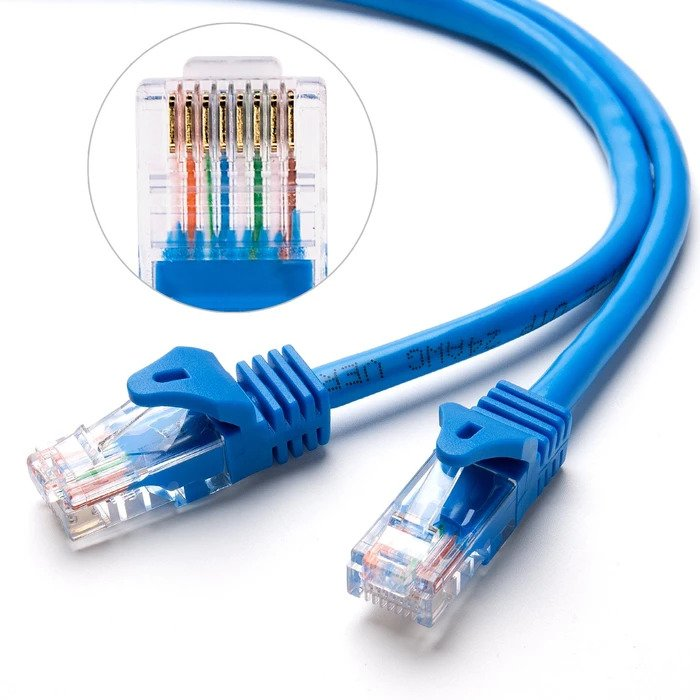
\includegraphics[width=.6\linewidth]{images/ethernet.jpg}
    \caption{An Ethernet cable used to network computers together.}
    \label{fig:ethernet}
\end{figure}

The other primary link layer technology is 802.11, more commonly known as Wi-Fi. With a wired network, signals can be sorted into separate wires so they don't overlap, but over a wireless network signals are broadcast and have the potential to interfere with one another. In order to prevent this, Wi-Fi is designed to allow devices to operate at slightly different frequencies which are arranged into channels.

There are two major variants of Wi-Fi: 2.4 gigahertz (GHz) and 5 GHz. These are two different frequency bands. Within each of them there are multiple channels. At 2.4 GHz, which was the first frequency available for Wi-Fi, there are 11 channels. However, the channels overlap with one another, so it is best for devices to use channels 1, 6, and 11, reducing the efffective number of channels down to 3. The newer 5 GHz protocol alleviates this problem by making hundreds of channels available. Most new devices can operate at either 2.4 GHz or 5 GHz, but some older devices only support 2.4 GHz.

The details of link layer technologies are complex, but luckily you rarely have to deal with them directly. In most cases, Ethernet or Wi-Fi have been engineered to the point where little effort is required to make them work properly, and you can focus on other layers of the network while trusting that signals are being carried appropriately by the link layer.


\section{Network Security}\label{sec:network:security}

One of the most important issues with computer networks is security. The Internet is frequently used for transmitting confidential messages, facilitating financial transactions, and other applications where security is paramount. For this reason,there are protocols dedicated to ensuring that the Internet can be secure. The most common such protocol is Transport Layer Security (TLS), which is a successor to an older protocol called Secure Sockets Layer (SSL). TLS is implemented at the transport layer of a network. Web traffic which uses TLS/SSL security is sent using the HTTPS protocol at the application layer, rather than the unsecured HTTP protocol.

Another common network security application is a Virtual Private Network, or VPN. A VPN allows computers connected to different LANs to communicate over the Internet as if they belonged to the same LAN. This is often used by companies to allow employees to access private resources even when they are away from the office. Security is very important for a VPN, and it can be provided using TLS or other protocols.

The details of TLS are complicated, and we will not get into them here. Instead, we will cover what exactly security means in a network setting, and look at three goals of any secure network: privacy, authenticity, and reliability. Achieving these goals requires using tools from cryptography, which you may learn about in a future course.

\subsection{Privacy}

When two parties want to securely transmit a message, one of their most straightforward goals is privacy. The two parties do not want a third party to be able to lisen in on their communication.

Following a standard convention in cryptography, we will denote the two parties by Alice and Bob, and the adversarial third party by Carol. Alice is sending a message to Bob, and Carol wants to listen in. Since network signals travel over cables, Carol could listen in to the signal by physically tapping into a wire. Even more easily, on a wireless network, all signals are broadcast over the air and can be received by anyone who wants to listen.

In order to protect their messages from being read by Carol, Alice and Bob use an encryption algorithm. Alice and Bob have some shared key, and when Alice wants to send a message, she first uses her key to turn the plain text of the message into a cipher text. If the algorithm is secure, then the cipher text cannot be converted back to the plain text without knowledge of the key. This way, if Carol manages to read the message, she will only see nonsensical cipher text. Only Bob, who has the key, can produce the plain text.

A key issue here is how Alice and Bob come to have the same key. If Alice tells Bob her key over the network, then Carol could retrieve the key and use it to decrypt all future messages. This is a fundamental problem in cryptography called the key-sharing problem. It is solved using a technique called public key cryptography. In TLS, public key cryptography is implemented using either the RSA algorithm, or a more sophisticated method called elliptic curve cryptography (ECC). These algorithms allow Alice and Bob to generate shared keys which Carol cannot intercept.

\subsection{Authenticity}

Even if Carol cannot read messages sent between Alice and Bob, she can still do damage. One potential attack would be for Carol to impersonate Alice, by sending a message to Bob which says it comes from Alice. This is why TLS must also protect the authenticity of messages: if a message says it comes from Alice, Bob needs some way of verifying that this is actually the case.

The public key cryptography algorithms used for ensuring privacy can also provide authenticity. In these algorithms, every party on the network has a private key which is never shared with anyone. This private key is important for generating the shared keys used for encrypting messages. It can also be used to generate a ``digital signature,'' which could only be produced by someone in possession of the private key. As long as the private key has never been shared, a digital signature can provide a guarantee of authenticity.

\subsection{Integrity}

Finally, even if Carol cannot read messages or impersonate Alice or Bob, she could try to modify one of their messages. This is called a man-in-the-middle (MITM) attack, where Carol intercepts Alice's communications, edits them, and then forwards them to Bob with Alice's signature intact.

To protect against this, TLS uses a message authentication code (MAC) which is sent along with any message. This is a short code sent with the message, which depends on the shared key and on the message. If the algorithms are secure, then it should be nearly impossible to generate a MAC without knowledge of both the shared key and the message. When Bob receives the message along with the MAC, he verifies that the MAC is correct. If it is not, then he knows the message has been altered in transit and discards it.

\subsection{Security versus Trust}

An enormous amount of expertise, testing, and iteration has gone into making TLS secure. However, it is still relatively common to hear about security problems on the Internet. Where do these problems come from?

In this context, it is important to recognize a key difference between security and trust. Network security provided by TLS achieves the three goals outlined above: privacy, authenticity, and integrity. When Alice communicates with Bob, she can be sure that only Bob can read her messages, that messages she receives from Bob really come from Bob, and that the messages have not been altered in transit. However, \emph{TLS does not guarantee that Alice can trust Bob}.

There are many ways in which Bob could be unreliable. For example, Bob could be attempting to execute a phishing attack by impersonating someone else. TLS guarantees that Bob cannot truly impersonate \ic{facebook.com}, but he could own \ic{fcebook.com} and, using TLS security, provide a website that looks just like \ic{facebook.com} and asks for your login credentials. If you provide them to \ic{fcebook.com}, then Bob could read your password and log into your actual Facebook account.

Even if Bob is not malicious, he could be irresponsible. For example, if Bob runs an online vendor which collects credit card information to make payments, it is crucial that Bob takes appropriate security measures on his local network to protect that credit card information from becoming known to an attacker. TLS does not guarantee that Bob has taken the necessary precautions. Many of the most substantial security problems arise on the Internet when many customers have trusted a vendor like Bob with their personal details like credit card numbers, and Bob suffers a data breach, putting this data into the wrong hands.

Network security is an evolving field as companies and governments work to protect against these sorts of vulnerabilities. There are many opportunities for employment in this area, as organizations increasingly need to rely on dedicated security professionals in order to keep their data and their clients' data safe.

\exercisesection

\begin{exercise}
    Put the following layers in order from top to bottom, and give an example of a protocol or technology used in each layer.
    \begin{itemize}
        \item Transport Layer
        \item Link Layer
        \item Application Layer
        \item Internet Layer
    \end{itemize}
\end{exercise}

\begin{exercise}
    What protocol is used as part of HTTPS in order to ensure secure transmission of data? List the three goals of this protocol and give a description of the kind of attack each goal seeks to prevent. Then give an example of an attack which would not be prevented by this protocol.
\end{exercise}

\begin{exercise}
    Identify all of the following blocks of IP addresses which contain 48.192.72.86. (\emph{Hint:} you may want to write out each address block in binary.)
    \begin{itemize}
        \item 48.192.0.0/12
        \item 48.192.0.0/16
        \item 48.192.0.0/20
        \item 48.0.0.0/4
        \item 48.0.0.0/8
        \item 48.0.0.0/12
        \item 48.192.64.0/20
        \item 48.192.64.0/24
    \end{itemize}
\end{exercise}

\begin{exercise}
    In a TCP handshake, Alice initiates by sending $\boxed{\ic{SYN}\ 895}$ to Bob. Give an example of the remaining steps that could take place in this handshake.
\end{exercise}

\begin{exercise}
    What is the main advantage of 5 GHz WiFi over 2.4 GHz WiFi? Why is 2.4 GHz WiFi still in use?
\end{exercise}